\chapter{4. Overview of Design and Contributions}

The are three main goals with the learnAir project.  The first is (1) to evaluate the usefulness and feasibility of applying machine learning algorithms to air quality sensor networks.  Specifically, this means testing whether we can predict when a low-cost sensor is giving reliable data based on the conditions under which it is measuring. The second goal is (2) to prototype a data solution that addresses the needs of the air quality sensing community-- particularly, the creation of an ecosystem that supports the needs of participants from high-end research facilities to lower-accuracy citizen projects-- and allows seamless, easy interaction between them.  It also must support the machine learning algorithms validated as part of our first goal in a scalable, automatic way (leveraging on-board, contextual sensors like temperature to help ground the data from its own air quality sensors).  Finally, we want (3) to prototype an actual, handheld system that uses the algorithms from (1) and the database from (2) to realize a deployable, useful mobile sensor system that demonstrates the concepts and ideas put forth in this thesis.  We believe this device will serve as a powerful rhetorical tool and push the dialog forward in citizen sensing communities.  We also believe this system will give improved data reliability and as a result a more accurate estimate of personal pollution exposure compared to comparably priced and spec'ed systems.      

The final system will enable a sensor to learn about itself when it is near a higher quality reference.  It will apply that knowledge to new measurements made under new conditions, even as it moves away from the reference system.  Every measurement the system makes will be accompanied by a simple prediction-- was this measurement accurate or not?  Every prediction will also come with an estimate of certainty-- how confident are we this prediction is accurate?  As more sensors of the same make and model are added to the network, predictions will improve and prior predictions can be revised.

\section{Machine Learning Validation}

Sensor technology-- especially in the air quality space-- is getting cheaper and more reliable.  For the first time, well-respected sensors are starting to appear in the \$100 range.  However, there are limitations on what is possible with small, affordable technology.  For example, electrochemical gas sensors break down in known ways-- their reactions are temperature, pressure, and humidity dependent, in some cases they are cross-sensitive to other gases, and their reactions have time-constants and noise susceptibility based on electrode size and exposure area.  Optical particulate sensors are frequently designed to mitigate external effects by applying (expensive) precise air flow control, heated inlets to eliminate fog, size-selective particle filtering, and advanced optics.

Sensors that break down in systemic ways may provide very reliable information under certain conditions.  While it may be obvious if a sensor has a single, well-understood failure mode (for instance, an optical sensor that is very reliable unless there is fog), compounded failure modes are more common and more difficult to infer.  By applying machine learning to this problem, we can automatically characterize which and how strongly underlying features are predictive of systematic errors.  

Machine learning has a strong likelihood for providing insight into sensor reliability assuming the sensors are not spurious: that their failures come predictably.  This assumption has likely not been true in the past, but the evidence suggests that we've entered into a new era of cheap air quality sensing-- where some devices are based on trustworthy, strong designs, but cost constraints have prevented the inclusion of a controlled environment typical for instrument level devices.  In these cases, we can measure the conditions instead of controlling them, and make an educated prediction about the reliability of any measurement.      

To test this theory, we built a stationary device that can measure ambient conditions (temperature, light, humidity, wind) and included a range of cheap air quality sensors for CO, NO2, O3, and particulate.  This sensor is called 'learnAir V1'.  This sensor was installed for ~2 months at a Mass Department of Environmental Protection (MassDEP) measurement site next to the inlet for reference EPA measurement equipment.  The data collected from our measurements were compared to the EPA reference data as a 'ground truth' reference, to characterize when the sensors were reading accurately and when they weren't.  We then used machine learning techniques to predict when the sensor was giving accurate readings or not. Using cross-validation techniques (splitting our collected data into a training set and a testing set), it is possible to characterize how well our algorithms predict sensor accuracy.  See Chapter 5 for a description of the device and MassDEP reference hardware, and Chapter 7 for an in-depth analysis of the machine learning techniques and cross-validation results.      
 
\section{ChainAPI Instance and Tools}

The air quality research community is actively working to mitigate the complications involved with inter-organization data-sharing.  Furthermore, they are interested and actively engaged in questions around the citizen sensing movement-- how should they inform and involve citizens in the air quality monitoring community?  How should they validate cheap consumer devices?  Is there a research use for the lower-quality data gathered from these networks, and how can they access and interact with it? 

Another contribution of this thesis is to build and adapt an example of ChainAPI-- a hypermedia data-sharing framework-- for use with air quality data.  ChainAPI offers many interesting advantages for sensor deployments as a thin, distributed hypermedia layer for linking data resources.  It provides unique advantages for a diverse, distributed ecosystem where different sub-communities can co-exist.  

In addition to creating a new ontology for air quality resources and building a development ChainAPI server, several new tools are necessary to interact with the ChainAPI air quality ecosystem.  The infrastructure built for this thesis provides automatic resource discovery and dataset creation-- so researchers can automatically find and interact with new datasets based on the type of data they are interested in working with, without \textit{a priori} knowledge of where to look for that data.  Its tools provides separation of concerns, so that raw data and data processing scripts are separated, instead of pre-processing occuring in an opaque way before data upload.  Its processing scripts-- that crawl through ChainAPI and update data-- offer transparency to data quality and data manipulation.  

This topology allows experts with certain sensors or devices to create, own, and update the processing elements for their technologies, and provide automatic, high-quality processing to novice users.  It provides the opportunity to create scripts that crawl through datasets looking for anomalies, out-of-spec operating characteristics, or out-of-service parts, and warn the device owners or data users.  Finally, it offers the ability to create learning algorithms that automatically improve as more data is added to the ChainAPI ecosystem. 

This contribution is an example of how ChainAPI could be adapted for air quality data sharing.  It includes a new ontology based on the needs of the air quality community, and a large suite of tools that make ChainAPI a scalable, powerful tool for dynamic, growing data ecosystems.  It also forms the basis for a truly automatic implementation of our machine learning algorithms.  See Chapter 6 for an in depth discussion of the contributions around ChainAPI.

\section{A Provocative Example}

Based on the infrastructure developed with ChainAPI and the algorithms tested at the EPA site, the final goal of the project is to build a fully functional, portable device that integrates all of these features.  There are several motivations for this: (1) as a rhetorical tool that can engage the citizen sensing community in a dialog about sensor data quality and validation, (2) as a means for deploying successful results from the previous sections as a best-in-class, trustworthy, manufacturable device, and (3) as a tool and platform for future testing of mobile use cases without having to do extensive data processing and manipulation by hand.  Once this system is built, the machine learning results and comparisons can be generated easily and automatically as long as the data is available in the ChainAPI ecosystem.

Two portable prototypes were designed and built as part of this thesis-- called 'learnAir V2' and 'learnAir V3'.  Both are battery powered, hand-held devices that integrate AlphaSense electrochemical and particulate sensors.  Both connect to a smartphone over BLE and push their data up to ChainAPI using GPS data from the phone application.  Both monitor ambient conditions of their measurements (vibration, temperature, humidity, light, wind) to help predict their accuracy.  

The two versions are very similar-- the main difference is the core microcontroller.  Version 2 is based on the Atmel ATmega32u4, and was programmed using the Arduino environment.  Version 3 is based on the lower-power, fully-featured STMicro STM32L152, which requires a more complicated build process, and comes with less library support.  There are cost and power savings associated with Version 3 (making it more 'production-worthy'), but functionally they are nearly identical solutions.  See Chapter 5 for an in-depth discussion of this hardware.



















%here's text referencing the (Table \ref{tab:sample_table}).
%
%\begin{table}
%  \centering
%  \begin{tabular}{l l l l l}
%    Column A & Column B & Column C & Column D & Column E \\
%    \toprule
%    A & B & C & D & E
%  \end{tabular}
%  \caption{A meaningless table}
%  \label{tab:sample_table}
%\end{table}

%Here's text referencing the margin figure (Figure \ref{fig:spin_margin}).
%
%\marginnote{\textbf{Margin Note:} Check it out, here's a margin note.}
%
%\begin{marginfigure}[{-10cm}]
% 	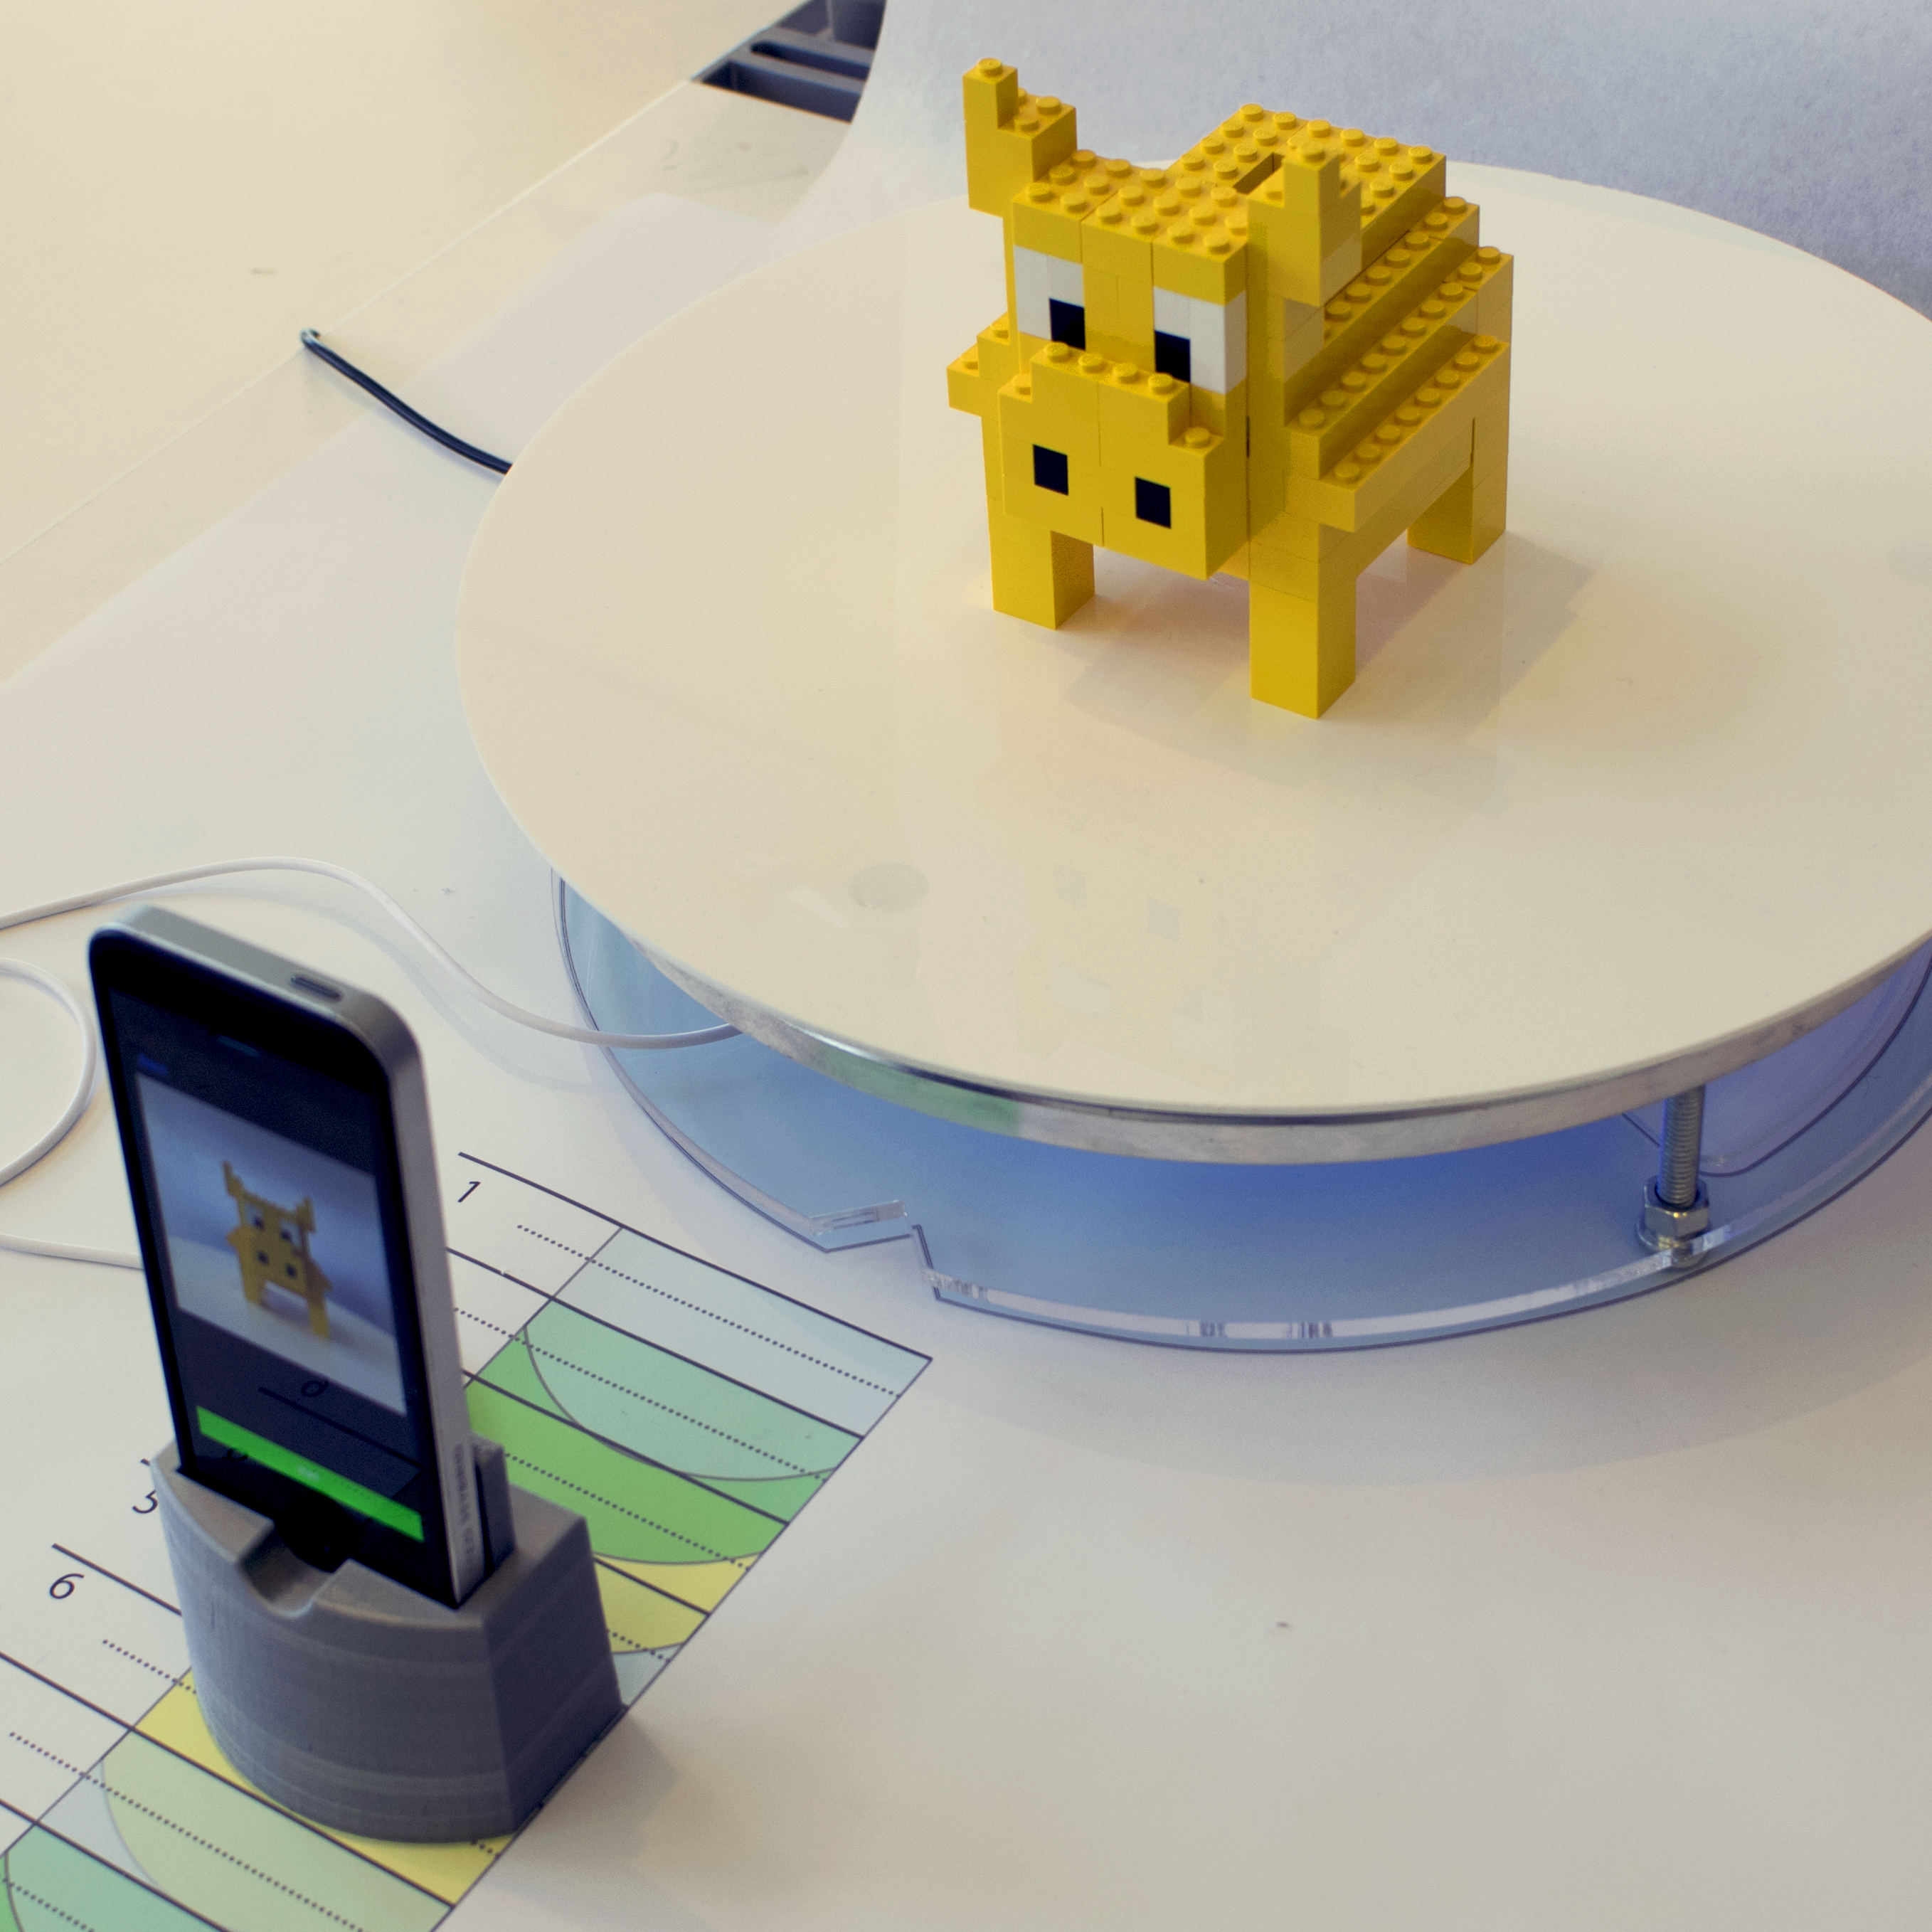
\includegraphics[width=\textwidth]{chap1/spin}               
% 	 \caption{Check it out, it's a Spin margin figure \url{spin.media.mit.edu}}
%  	\label{fig:spin_margin}
%\end{marginfigure}

%\begin{figure}[htb]
% 	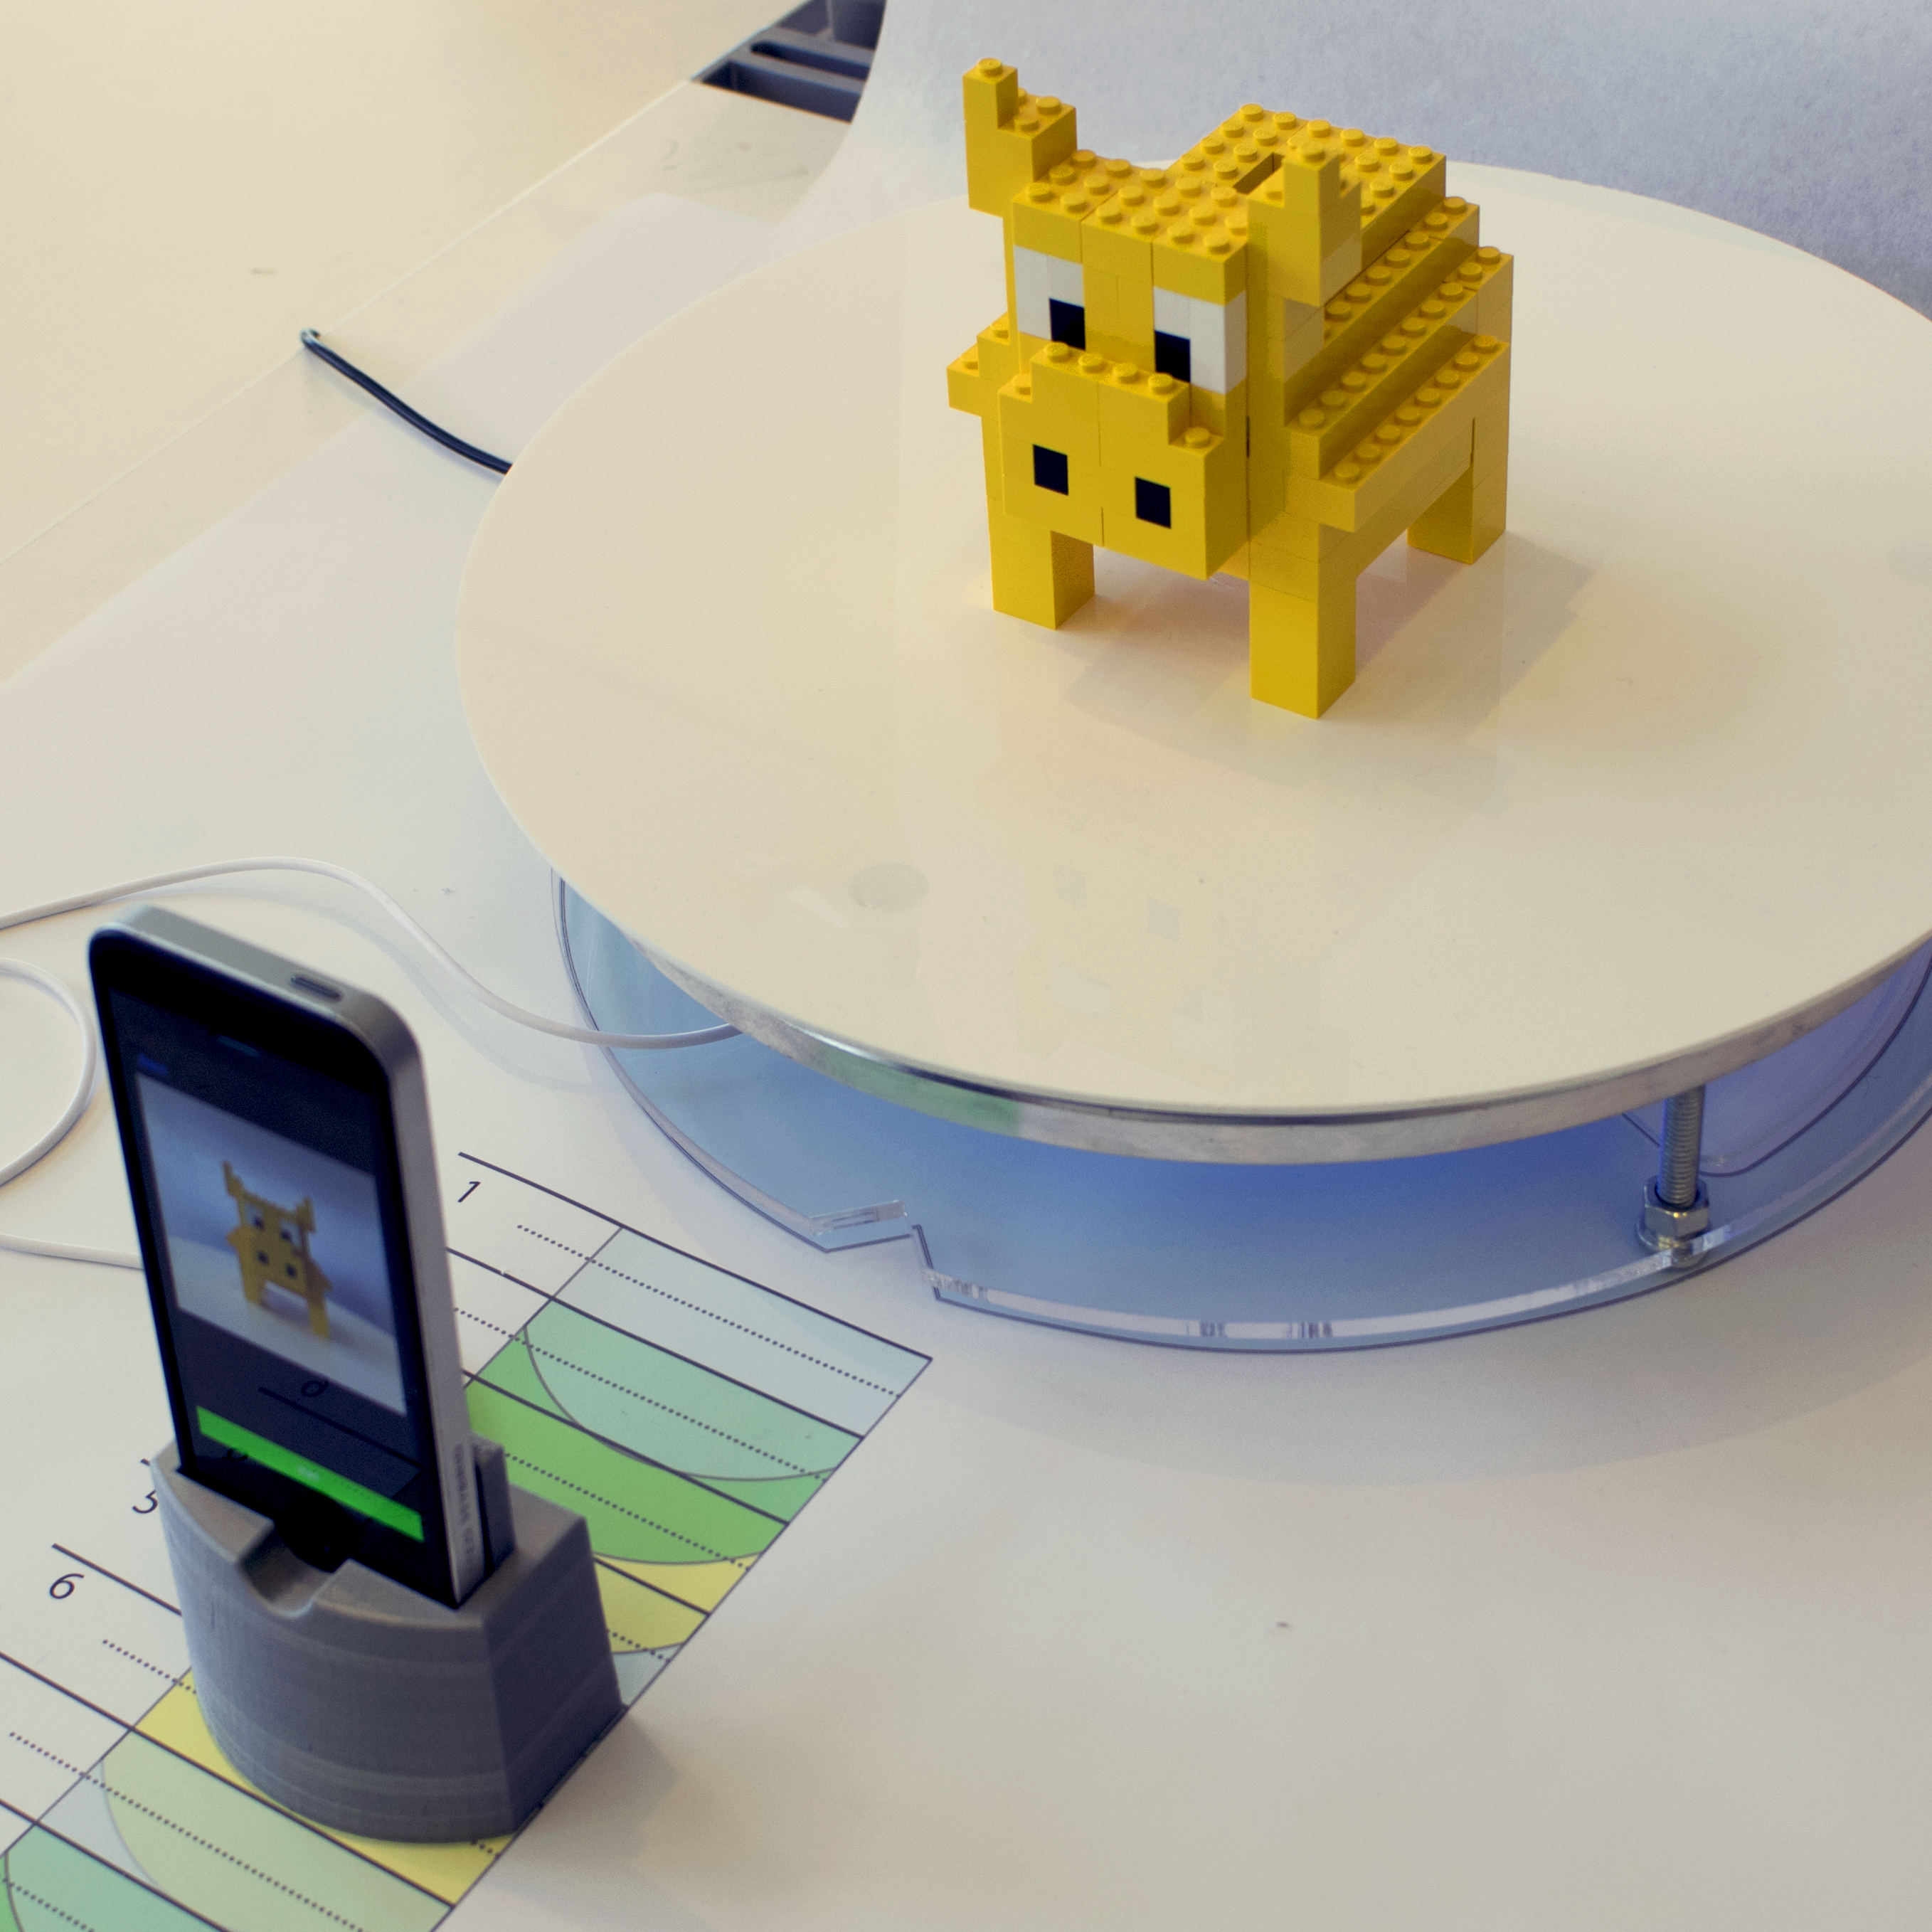
\includegraphics[width=\textwidth]{chap1/spin}               
% 	 \caption{Check it out, it's a Spin \url{spin.media.mit.edu}}
%  	\label{fig:spin}
%\end{figure}